\documentclass[convert={density=1200,size=1080x800,outext=.png}, tikz]{standalone}
\usetikzlibrary{matrix}
\usetikzlibrary{angles, quotes}
\usetikzlibrary{plotmarks}
\usetikzlibrary{arrows.meta}
\usetikzlibrary{positioning}
% \usetikzlibrary{arrows.meta}
\begin{document}
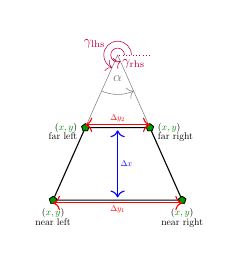
\begin{tikzpicture}

  \matrix (grid) [matrix of nodes, transparent=1]
  {
    8 & 8 & 1 & 6 & 6 \\
    3 & 3 & 5 & 7 & 7 \\
    4 & 4 & 9 & 2 & 2 \\
    4 & 4 & 9 & 2 & 2 \\
    4 & 4 & 9 & 2 & 2 \\
  };

  % runway outline
  \draw (grid-5-1.center)
  to (grid-3-2.center)
  to (grid-3-4.center)
  to (grid-5-5.center)
  to cycle;


  % runway extensions
  \draw[gray, very thin]
  (grid-3-2.center) coordinate (A) to
  (grid-1-3.center) coordinate (B) to
  (grid-3-4.center) coordinate (C)
  pic ["$\alpha$"scale=0.5, draw, solid, ->] {angle};
  % \draw[gray, dashed, very thin, shorten <=1pt] (grid-3-4.center) to (grid-1-3.center);

  \draw[purple, very thin, densely dotted, opacity=1] (grid-1-4.center) to (grid-1-3.center);
  \draw[purple, very thin, densely dotted, opacity=0]
  (grid-1-4.center) coordinate (A) to
  (grid-1-3.center) coordinate (B) to
  (grid-3-2.center) coordinate (C)
  pic ["$\gamma_{\rm lhs}$"{scale=0.5, anchor=east}, draw, solid, ->, angle radius=5.0, angle eccentricity=1.0, opacity=1] {angle};

  \draw[purple, very thin, densely dotted, opacity=0]
  (grid-1-4.center) coordinate (A) to
  (grid-1-3.center) coordinate (B) to
  (grid-3-4.center) coordinate (C)
  pic ["$\gamma_{\rm rhs}$"{scale=0.5, anchor=north west}, draw, solid, ->, angle radius=2.5, angle eccentricity=-0., opacity=1] {angle};


  % corner coordinates.
  \draw (grid-5-1.center) node[green!60!black, scale=0.7] {\pgfuseplotmark{pentagon*}} node[black, scale=0.7] {\pgfuseplotmark{pentagon}};
  \draw (grid-5-5.center) node[green!60!black, scale=0.7] {\pgfuseplotmark{pentagon*}} node[black, scale=0.7] {\pgfuseplotmark{pentagon}};
  \draw (grid-3-2.center) node[green!60!black, scale=0.7] {\pgfuseplotmark{pentagon*}} node[black, scale=0.7] {\pgfuseplotmark{pentagon}};
  \draw (grid-3-4.center) node[green!60!black, scale=0.7] {\pgfuseplotmark{pentagon*}} node[black, scale=0.7] {\pgfuseplotmark{pentagon}};

  \node[below=0.1 of grid-5-1.center, scale=0.35, inner sep=0pt] (corner-label-nl){\((\textcolor{green!50!black}{x, y})\)};
  \node[below=0 of corner-label-nl, scale=0.35, inner sep=0pt] {near left};

  \node[below=0.1 of grid-5-5.center, scale=0.35, inner sep=0pt] (corner-label-nr){\((\textcolor{green!50!black}{x, y})\)};
  \node[below=0 of corner-label-nr, scale=0.35, inner sep=0pt] {near right};

  \node[left=0.1 of grid-3-2.center, scale=0.35, inner sep=0pt] (corner-label-fl){\((\textcolor{green!50!black}{x, y})\)};
  \node[below=0 of corner-label-fl.south east, scale=0.35, inner sep=0pt, anchor=north east] {far left};

  \node[right=0.1 of grid-3-4.center, scale=0.35, inner sep=0pt] (corner-label-fr){\((\textcolor{green!50!black}{x, y})\)};
  \node[below=0 of corner-label-fr.south west, scale=0.35, inner sep=0pt, anchor=north west] {far right};

  % alongtrack distance
  \draw[blue, <->, shorten >=1pt, shorten <=1pt] (grid-5-3.center) to
    node[right, scale=0.3] {$\Delta x$}
    (grid-3-3.center);

  % crosstrack distance near and far
  \draw[red, <->]
    ([yshift=-1pt]grid-5-1.center) to
    node[below, scale=0.3] {$\Delta y_{1}$}
    ([yshift=-1pt]grid-5-5.center);
    \draw[red, <->] ( [yshift=+1pt]grid-3-2.center) to
        node[above, scale=0.3] {$\Delta y_{2}$}
        ([yshift=+1pt]grid-3-4.center);


\end{tikzpicture}
\end{document}
